% Optimized FPGA Acceleration of YOLOv8 Detection Head
% Springer LNCS (svproc) for IAAA
%
%%%%%%%%%%%%%%%% Springer %%%%%%%%%%%%%%%%%%%%%%%%%%%%%%%%%%

\documentclass{svproc}

% Recommended packages
\usepackage{url}
\usepackage{graphicx}
\usepackage{amsmath}
\usepackage{amssymb}
\usepackage{booktabs}
\usepackage{multirow}
\usepackage{array}
\usepackage{xcolor}
\definecolor{slate50}{HTML}{FFFFFF}   
\definecolor{slate100}{HTML}{FFFFFF}  
\definecolor{slate200}{HTML}{FFFFFF}  
\definecolor{slate300}{HTML}{FFFFFF}  
\definecolor{slate600}{HTML}{000000}  
\definecolor{slate800}{HTML}{000000}  
\definecolor{slate900}{HTML}{000000}  
\usepackage{float}
\usepackage{pifont}
\usepackage[section]{placeins}
\usepackage{tikz}
\usetikzlibrary{shapes.geometric, arrows.meta, positioning, calc, decorations.pathreplacing, fit, patterns}
\graphicspath{{figures/}}
\def\UrlFont{\rmfamily}

% Tighten float spacing to prevent page overflow
\setlength{\intextsep}{6pt plus 2pt minus 2pt}     
\setlength{\textfloatsep}{8pt plus 2pt minus 2pt}   
\setlength{\floatsep}{6pt plus 2pt minus 2pt}       
\setlength{\abovecaptionskip}{4pt}                   
\setlength{\belowcaptionskip}{2pt}                   
\emergencystretch=1em

\begin{document}
\raggedbottom
\mainmatter

%=====================================================================
\title{Optimized FPGA Acceleration of YOLOv8 Detection Head for Resource-Constrained UAVs}

\titlerunning{FPGA Accelerator for the YOLOv8 Detection Head}

\author{Nguyen Vo \and Dang Tran \and Binh Vo}

\authorrunning{Nguyen Vo et al.}

\tocauthor{Nguyen Vo, Dang Tran, Binh Vo}

\institute{%
Ho Chi Minh City University of Technology (HCMUT),\\
Vietnam National University Ho Chi Minh City (VNU-HCM)\\
\email{\{nguyen.vohoang, dang.tran686868, binh\}@hcmut.edu.vn}}

\maketitle

%=====================================================================
% ABSTRACT
%=====================================================================
\begin{abstract}
UAV-deployed object detectors must satisfy strict Size, Weight, and Power (SWaP) constraints, yet anchor-free models like YOLOv8 introduce severe post-processing bottlenecks, specifically within Distribution Focal Loss (DFL) coordinate decoding and Non-Maximum Suppression (NMS) spatial filtering. Standard Field Programmable Gate Array (FPGA) implementations routinely offload these operations to a host CPU, resulting in memory-transfer penalties that degrade real-time inference. We therefore propose a resource-efficient, fully hardware-integrated YOLOv8 Detection Head accelerator. Specifically, we process all six convolutional layers through a single time-shared MAC engine, decode coordinates via a zero-DSP Look-Up Table (LUT) unit, and filter overlapping bounding boxes by replacing iterative dividers with a parallel algebraic cross-multiplication pipeline. Experimental results on the Xilinx Zynq-7020 platform confirm that the proposed accelerator eliminates the CPU post-processing bottleneck, sustaining a consistent 32.1\,FPS at 67.0\% $\text{mAP}_{50}$ on the KIIT-MiTA dataset within a 0.302\,W power envelope using only 10 DSP blocks.

\keywords{FPGA, YOLOv8, hardware architecture, DFL, division-free NMS, UAV, INT8}
\end{abstract}

%=====================================================================
% 1. INTRODUCTION
%=====================================================================
\section{Introduction}
\label{sec:intro}

Real-time object detection algorithms deployed on Unmanned Aerial Vehicles (UAVs) must operate within strict Size, Weight, and Power (SWaP) constraints~\cite{yolo_uav2023,chakrabarty2025kiitmita,personnel_sar2025}. Unlike legacy anchor-based networks (e.g., YOLOv5, YOLOv7) that exhibit limited adaptability to multi-scale drone perspectives, modern anchor-free models such as YOLOv8~\cite{ultralytics2023yolov8} currently achieve state-of-the-art precision. While subsequent software iterations (e.g., YOLOv10, YOLOv11) propose architectural adaptations, YOLOv8 represents the first widely-adopted anchor-free YOLO design requiring hardware DFL decoding, making it the natural architectural target for this work. This anchor-free design, however, introduces significant algorithmic complexity for fixed-point hardware circuitry. Extracting bounding-box coordinates requires non-linear floating-point exponentials and normalization division for Distribution Focal Loss (DFL) vector decoding~\cite{li2020generalized}, while the mandatory Non-Maximum Suppression (NMS) algorithm conventionally relies on iterative hardware dividers to evaluate the Intersection over Union (IoU) of overlapping bounding-box candidates.

Existing Field Programmable Gate Array (FPGA) accelerators~\cite{saidani2024hardware,essel2025yolov8fpga} typically prioritize convolutional backbone acceleration, frequently offloading the complex DFL and NMS operations to an embedded Central Processing Unit (CPU) host. Even recent hardware designs explicitly targeting the YOLOv8 Detection Head restrict optimization to architectural modifications (e.g., grouped channel convolutions)~\cite{guan2024yolov8}, leaving the CPU-memory transfer bottleneck unresolved. The resulting latency penalty is substantial. For instance, Danilowicz et al.~\cite{danilowicz2025sort} empirically demonstrated that a generic YOLOv8 FPGA backbone sustaining 195\,FPS is bottlenecked to 24\,FPS purely due to host-delegated anchor-free NMS synchronization.

Simply offloading these modules to hardware in isolation, however, is insufficient. Integrating these standalone post-processing modules natively into Programmable Logic (PL) presents severe resource challenges. Bespoke NMS hardware pipelines historically rely on extensive hardware dividers~\cite{anupreetham2024nms} or large parallel LUT arrays~\cite{nguyen2021fast}, which rapidly scale DSP and logic capacities beyond the strict limits of Edge UAV deployments. Furthermore, in anchor-free architectures, DFL decoding must complete before NMS can evaluate candidate boxes---a strict sequential dependency that prevents isolated NMS cores from resolving the full post-processing bottleneck without integrated DFL acceleration.

To address these limitations, this paper introduces a resource-efficient, fully hardware-integrated YOLOv8 Detection Head architecture that eliminates the CPU data-transfer bottleneck. The core scientific contributions are:
\begin{enumerate}
    \item \textbf{Zero-DSP LUT-based Distribution Focal Loss (DFL) Decoder:} We propose a 5-stage integer pipeline replacing floating-point Softmax with a 256-entry BRAM Look-Up Table (LUT). This eliminates exponential logic, mapping the full DFL pipeline to precisely 539 LUTs and zero DSP slices.
    \item \textbf{Division-Free IoU Non-Maximum Suppression (NMS):} We reformulate the IoU calculation to use algebraic cross-multiplication, discarding hardware dividers in favor of a 4-DSP parallel integer multiplier architecture. This reduces the hardware footprint of NMS spatial filtering, enabling autonomous execution within the 220-DSP limit of the Zynq-7020.
    \item \textbf{Resource-Multiplexed Convolutional Neural Network (CNN) Datapath:} We introduce a time-shared parallel MAC engine that processes all six detection-head layers sequentially using 6 DSPs. Per-channel scale factors are fused directly into the hardware re-quantization path~\cite{jacob2018quantization}, avoiding floating-point corrections and entirely bypassing the CPU during inference bounding-box extraction.
\end{enumerate}

%=====================================================================
% 2. SYSTEM DESIGN
%=====================================================================
\section{System Design}
\label{sec:architecture}

Mapping the YOLOv8 detection head to a fixed-point FPGA entails routing a $40{\times}40$ feature map through two parallel paths: a bounding-box regression cv2 branch relying on DFL ($4{\times}16$ coordinate bins), and a classification cv3 branch, comprising six convolutional layers sequentially. Spatial-parallel instantiation of all six networks often exceeds the logic footprint of edge-class FPGAs. Fig.~\ref{fig:system_arch} illustrates our resource-efficient architecture, where the complete head executes autonomously within the PL, fully relieving the ARM Processing System (PS) of post-processing duties.

\begin{figure}[H]
\centering
\scalebox{0.75}{%
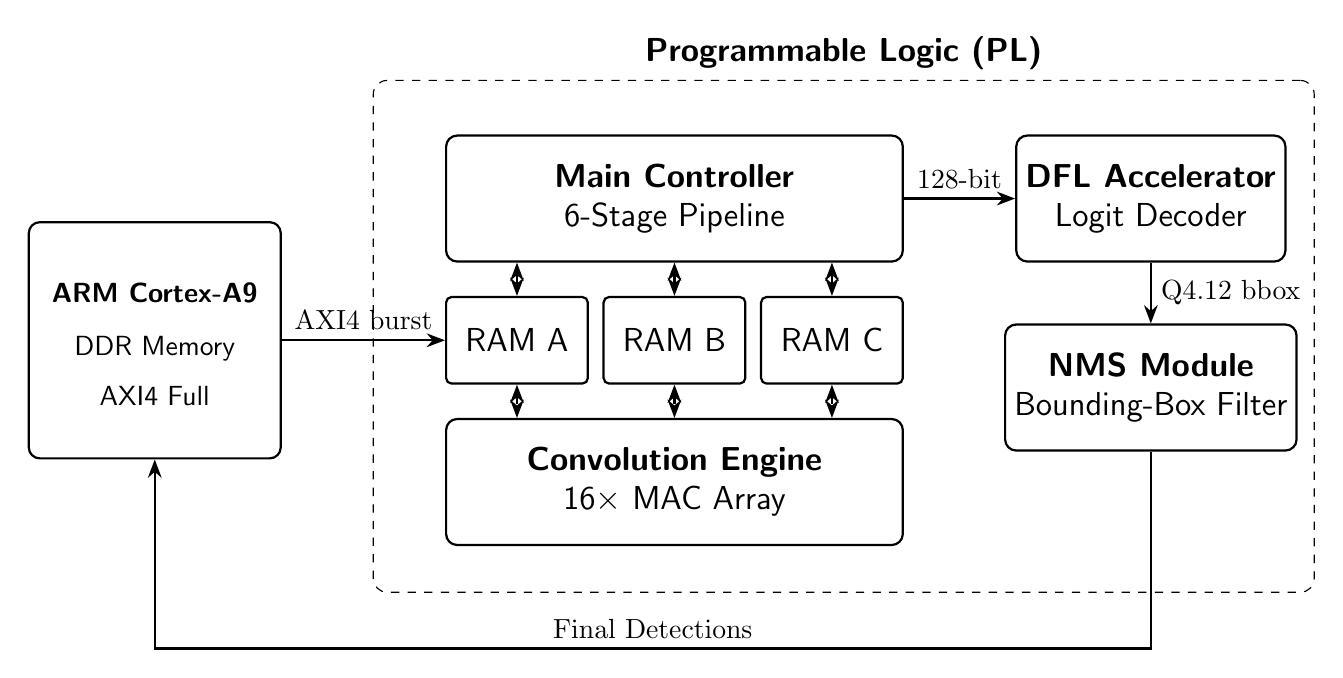
\begin{tikzpicture}[
    font=\sffamily\large,
    >=Stealth,
    draw=slate800, text=slate900,
    box/.style={draw=slate800, rounded corners=4pt, minimum width=3.5cm, minimum height=1.6cm, align=center, line width=0.8pt},
    mem/.style={draw=slate800, rounded corners=2pt, minimum width=1.8cm, minimum height=1.1cm, align=center, fill=slate200, line width=0.8pt},
    dsp/.style={draw=slate800, rounded corners=4pt, minimum width=4.5cm, minimum height=1.6cm, align=center, fill=slate100, line width=0.8pt},
]
\node[box, fill=slate50, minimum width=3.2cm, minimum height=3cm] (ps) at (-1.1, 0) {};
\node[font=\sffamily\normalsize\bfseries] at (-1.1, 0.6) {ARM Cortex-A9};
\node[font=\sffamily\normalsize] at (-1.1, -0.1) {DDR Memory};
\node[font=\sffamily\normalsize] at (-1.1, -0.7) {AXI4 Full};

\node[draw, dashed, inner sep=14pt, rounded corners=5pt, fill=white, minimum width=11.95cm, minimum height=6.5cm, label={[font=\sffamily\large\bfseries]above:Programmable Logic (PL)}] (pl) at (7.65, 0.05) {};

\node[box, fill=slate100, minimum width=5.8cm] (fsm) at (5.5, 1.8) {\textbf{Main Controller}\\6-Stage Pipeline};
\node[mem] (rama) at (3.5, 0) {RAM A};
\node[mem] (ramb) at (5.5, 0) {RAM B};
\node[mem] (ramc) at (7.5, 0) {RAM C};
\node[dsp, minimum width=5.8cm] (engine) at (5.5, -1.8) {\textbf{Convolution Engine}\\16$\times$ MAC Array};
\node[box, fill=slate100, minimum width=3cm] (dfl) at (11.55, 1.8) {\textbf{DFL Accelerator}\\Logit Decoder};
\node[box, fill=slate100, minimum width=3cm] (nms) at (11.55, -0.6) {\textbf{NMS Module}\\Bounding-Box Filter};

\draw[->, thick, draw=slate800] (ps.east) -- node[above, font=\normalsize] {AXI4 burst} (rama.west |- ps.east);
\draw[<->, thick, draw=slate800] (fsm.south) ++(-2.0,0) -- (rama.north);
\draw[<->, thick, draw=slate800] (fsm.south) -- (ramb.north);
\draw[<->, thick, draw=slate800] (fsm.south) ++(2.0,0) -- (ramc.north);
\draw[<->, thick, dashed, draw=slate800] (rama.south) -- (engine.north -| rama.south);
\draw[<->, thick, dashed, draw=slate800] (ramb.south) -- (engine.north);
\draw[<->, thick, dashed, draw=slate800] (ramc.south) -- (engine.north -| ramc.south);
\draw[->, thick, draw=slate800] (fsm.east) -- node[above, font=\normalsize] {128-bit} (dfl.west);
\draw[->, thick, draw=slate800] (dfl.south) -- node[right, font=\normalsize] {Q4.12 bbox} (nms.north);
\draw[->, thick, draw=slate800] (nms.south) -- ++(0,-2.5) coordinate (nmsdrop) -| node[above, font=\normalsize, pos=0.25] {Final Detections} (ps.south);
\end{tikzpicture}
}
\caption{System Architecture. The PL executes the complete detection head autonomously; the ARM PS only loads features and receives detections via AXI4 burst.}
\label{fig:system_arch}
\end{figure}

\subsection{Resource-Multiplexed CNN Engine}
To minimize the spatial footprint typical of unrolled hardware mappings, our architecture avoids redundant CNN layer instantiations. Instead, we implement a single reconfigurable \texttt{conv\_stage} supporting variable kernel sizes and channel counts managed by a global Finite State Machine (FSM). The FSM orchestrates execution sequentially ($\text{cv2\_0} \to \text{cv2\_1} \to \text{cv2\_2} \to \text{cv3\_0} \to \text{cv3\_1} \to \text{cv3\_2}$). Consecutive layer data hazards are accommodated via a 3-BRAM architecture: RAM A and B alternate as ping-pong input/output buffers between consecutive layers, while RAM C independently preserves the cv2 branch output during cv3 branch execution, preventing cross-branch data corruption.

As shown in Fig.~\ref{fig:pe}, the core datapath utilizes an Input Channel Stationary dataflow, routing a BRAM line-buffer into an array of 16 parallel Multiply-Accumulate (MAC) units. By mapping narrow fixed-point multiplications to LUT-based logic rather than hard DSP primitives, the engine restricts DSP utilization to 6 blocks, enabling a 512-bit parallel datapath mapped primarily to standard logic elements. Quantization scaling is implemented directly in hardware as:
\begin{equation}
    y = \text{clamp}\!\left(\!\left(\frac{(\text{acc} - z_{in}) \times M_{int}}{2^{S}}\right) + z_{out},\; -128,\; 127\right)
\end{equation}

\begin{figure}[H]
\centering
\scalebox{0.72}{%
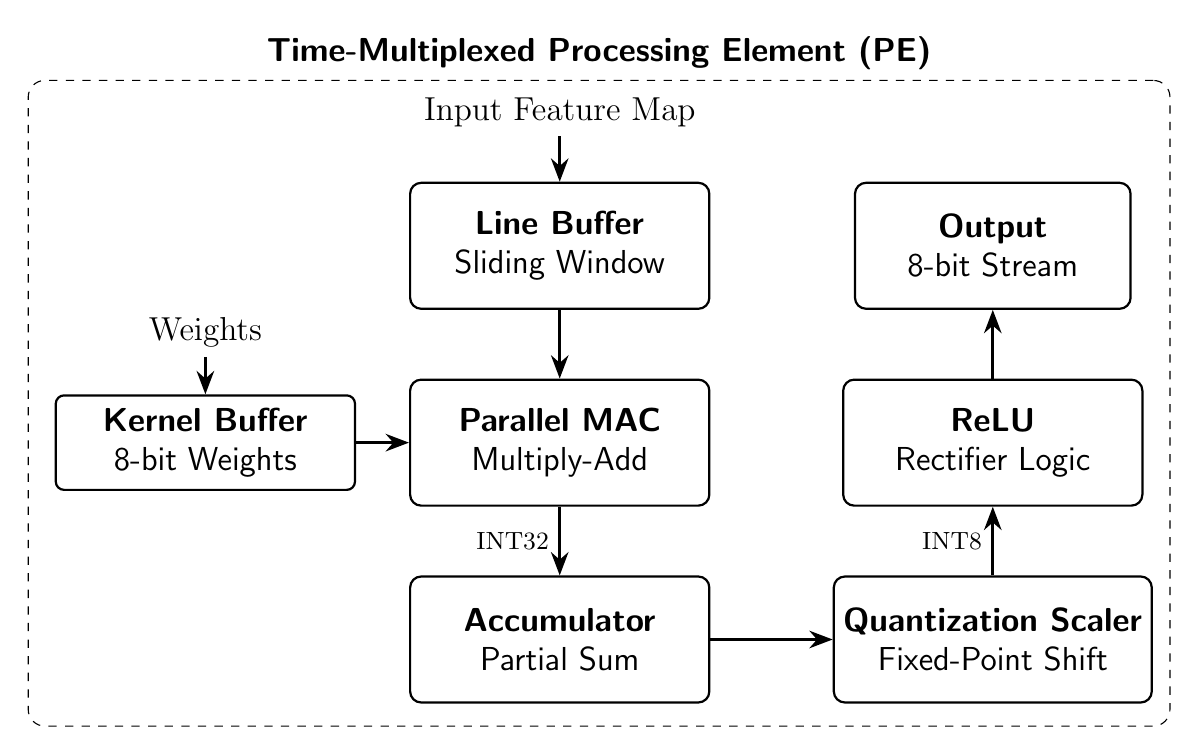
\begin{tikzpicture}[
    font=\sffamily\large,
    >=Stealth,
    draw=slate800, text=slate900,
    block/.style={draw=slate800, rounded corners=4pt, minimum width=3.8cm, minimum height=1.6cm, align=center, line width=0.8pt, fill=slate100},
    sram/.style={draw=slate800, rounded corners=3pt, minimum width=3.8cm, minimum height=1.2cm, align=center, line width=0.8pt, fill=slate200},
    ext/.style={draw=slate800, rounded corners=4pt, minimum width=3.8cm, minimum height=1.6cm, align=center, line width=0.8pt, fill=slate50},
    outblock/.style={draw=slate800, rounded corners=4pt, minimum width=3.5cm, minimum height=1.6cm, align=center, line width=0.8pt, fill=slate300},
]
% ── PE dashed bounding box ──
\node[draw, dashed, inner sep=18pt, rounded corners=6pt, fill=white,
      minimum width=14.5cm, minimum height=8.2cm,
      label={[font=\sffamily\large\bfseries]above:Time-Multiplexed Processing Element (PE)}]
      (pe) at (0.5, -2.0) {};

% ── External I/O Node ──
\node[font=\large] (in_node) at (0, 1.7) {Input Feature Map};

% ── Column 1 (Flow Downward) ──
\node[ext] (lb) at (0, 0) {\textbf{Line Buffer}\\Sliding Window};
\node[block] (mac) at (0, -2.5) {\textbf{Parallel MAC}\\Multiply-Add};
\node[block] (acc) at (0, -5.0) {\textbf{Accumulator}\\Partial Sum};

% ── Column 2 (Flow Upward) ──
\node[block] (rq) at (5.5, -5.0) {\textbf{Quantization Scaler}\\Fixed-Point Shift};
\node[block] (relu) at (5.5, -2.5) {\textbf{ReLU}\\Rectifier Logic};
\node[outblock] (output) at (5.5, 0) {\textbf{Output}\\8-bit Stream};

% ── Weight SRAM ──
\node[sram] (wsram) at (-4.5, -2.5) {\textbf{Kernel Buffer}\\8-bit Weights};
\node[font=\large] (pcw) at (-4.5, -1.1) {Weights};

% ── Arrows with Minimal Bit-Width Transition Labels ──
\draw[->, very thick, draw=slate800] (in_node) -- (lb);
\draw[->, very thick, draw=slate800] (lb) -- (mac);
\draw[->, very thick, draw=slate800] (pcw) -- (wsram);
\draw[->, very thick, draw=slate800] (wsram) -- (mac);
\draw[->, very thick, draw=slate800] (mac) -- node[left, font=\small] {INT32} (acc);
\draw[->, very thick, draw=slate800] (acc) -- (rq);
\draw[->, very thick, draw=slate800] (rq) -- node[left, font=\small] {INT8} (relu);
\draw[->, very thick, draw=slate800] (relu) -- (output);
\end{tikzpicture}
}
\caption{PE Microarchitecture. 16 parallel MAC units produce 512-bit output per cycle; re-quantization uses combinational logic without DSP primitives.}
\label{fig:pe}
\end{figure}

\subsection{Zero-DSP Hardware DFL Accelerator}
DFL converts 16 INT8 logits into a single fixed-point bounding-box coordinate. Directly mapping DFL to fixed-point hardware is non-trivial: the Softmax operation requires floating-point $e^x$ computation, which typically necessitates costly Taylor-series approximations consuming multiple DSP stages. We resolve this exponential bottleneck by replacing DSP-based Softmax computation with a single-cycle memory lookup sequence, and restricting the subsequent normalization division entirely to standard LUT logic (Fig.~\ref{fig:dfl_pipeline}). 

\begin{figure}[H]
\centering
\scalebox{0.72}{%
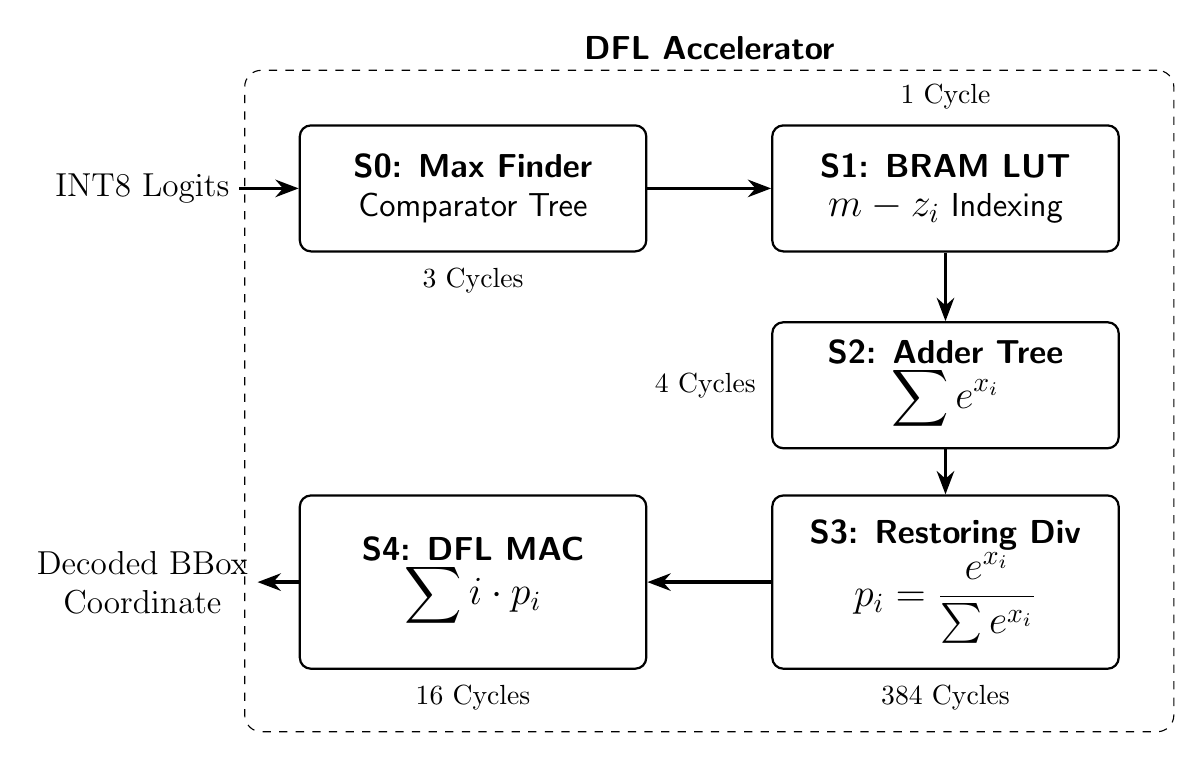
\begin{tikzpicture}[
    font=\sffamily\large,
    >=Stealth,
    draw=slate800, text=slate900,
    block/.style={draw=slate800, rounded corners=4pt, minimum width=4.4cm, minimum height=1.6cm, align=center, line width=0.8pt, fill=slate100},
    cycle/.style={font=\normalsize, text=slate600}
]

% ── Bounding Box ──
\node[draw, dashed, inner sep=18pt, rounded corners=6pt, fill=white,
      minimum width=11.8cm, minimum height=8.4cm,
      label={[font=\sffamily\large\bfseries]above:DFL Accelerator}]
      (bx) at (3.0, -2.7) {};

% ── External I/O ──
\node[font=\large] (in_node) at (-4.2, 0) {INT8 Logits};
\node[font=\large, align=center] (out_node) at (-4.2, -5.0) {Decoded BBox\\Coordinate};

% ── Top Row (Left to Right) ──
\node[block] (s0) at (0, 0) {\textbf{S0: Max Finder}\\Comparator Tree};
\node[cycle, below=2pt] at (s0.south) {3 Cycles};

\node[block] (s1) at (6.0, 0) {\textbf{S1: BRAM LUT}\\{\Large $m - z_i$} Indexing};
\node[cycle, above=2pt] at (s1.north) {1 Cycle};

% ── Middle Row (Right-Aligned) ──
\node[block] (s2) at (6.0, -2.5) {\textbf{S2: Adder Tree}\\{\Large $\displaystyle \sum e^{x_i}$}};
\node[cycle, left=2pt] at (s2.west) {4 Cycles};

% ── Bottom Row (Right to Left) ──
\node[block, minimum height=2.2cm] (s3) at (6.0, -5.0) {\textbf{S3: Restoring Div}\\{\Large $\displaystyle p_i = \frac{e^{x_i}}{\sum e^{x_i}}$}};
\node[cycle, below=2pt] at (s3.south) {384 Cycles};

\node[block, minimum height=2.2cm] (s4) at (0, -5.0) {\textbf{S4: DFL MAC}\\{\Large $\displaystyle \sum i \cdot p_i$}};
\node[cycle, below=2pt] at (s4.south) {16 Cycles};

% ── Arrows ──
\draw[->, very thick, draw=slate800] (in_node) -- (s0);
\draw[->, very thick, draw=slate800] (s0) -- (s1);
\draw[->, very thick, draw=slate800] (s1) -- (s2);
\draw[->, very thick, draw=slate800] (s2) -- (s3);
\draw[->, very thick, draw=slate800] (s3) -- (s4);
\draw[->, very thick, draw=slate800] (s4) -- (out_node);
\end{tikzpicture}
}
\caption{Five-stage DFL accelerator pipeline. S3 uses a restoring divider implemented in LUT logic, consuming zero DSP slices.}
\label{fig:dfl_pipeline}
\end{figure}

The 5-stage pipelined accelerator isolates the local maximum logit $m$ via a cascading comparator tree (S0) to prevent mathematical overflow ($e^{z_i - m}$). Stage 1 (S1) performs a single-cycle memory fetch against a 256-entry BRAM initialized with Q8.8 fixed-point exponential constants (8 integer bits, 8 fractional bits). This 256-entry depth covers the full value range of an 8-bit quantized logit ($z_{in} \in [0, 255]$), while the Q8.8 fractional format ensures sufficient bounding-box coordinate precision without exceeding a standard 18-bit BRAM width. Stages 2 and 3 accumulate the exponential values and normalize them via a restoring divider, confining operations to standard logic elements. This structure maps the bounding-box coordinate directly to a Q4.12 fractional integer (4 integer bits, 12 fractional bits) without consuming any DSP slices.
\subsection{Division-Free IoU NMS}
A primary computational bottleneck within standard NMS hardware pipelines is the Intersection over Union (IoU) calculation, which traditionally requires high-latency sequential hardware dividers. Our architecture eliminates this requirement by evaluating a division-free logical formulation:
\begin{equation}
    \text{suppress}(B_j) \;\Leftarrow\; \text{inter} \times D_{\text{IoU}} > \text{union} \times N_{\text{IoU}} \;\wedge\; \text{conf}(B_i) \geq \text{conf}(B_j)
\end{equation}
By cross-multiplying both sides of the IoU threshold inequality, division is eliminated entirely, replacing it with two integer multiplications.

\begin{figure}[H]
\centering
\scalebox{0.70}{%
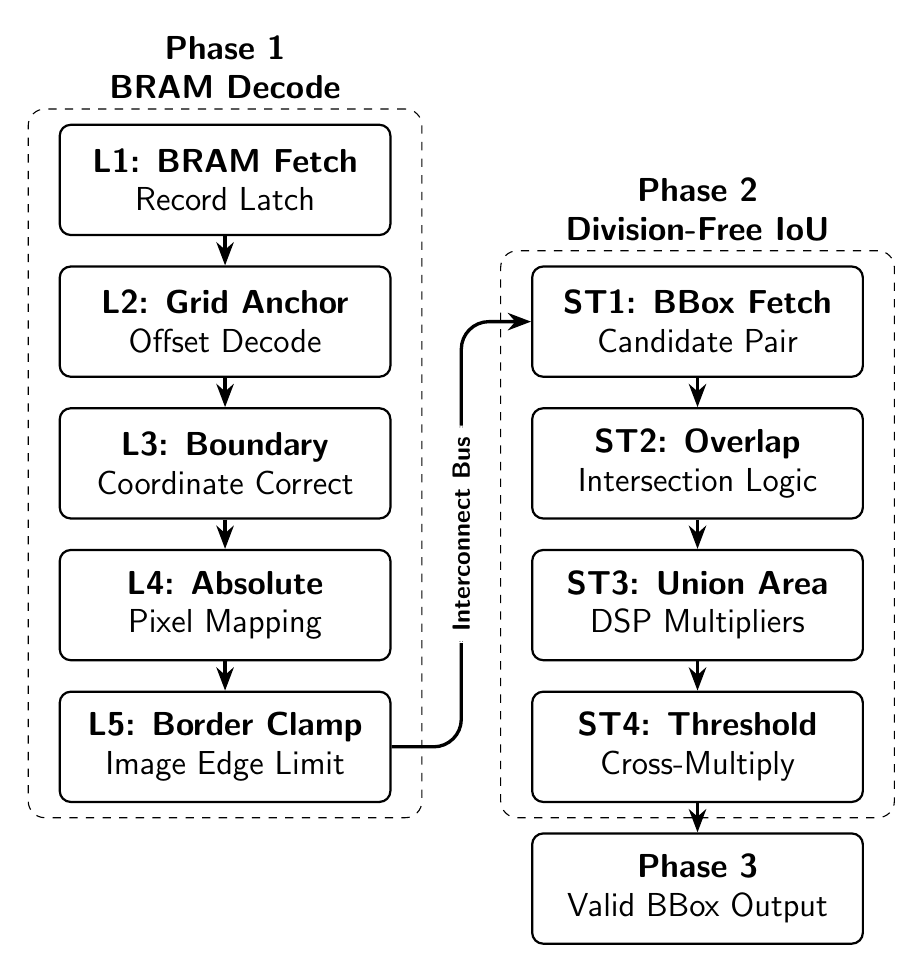
\begin{tikzpicture}[
    font=\sffamily\large,
    >=Stealth,
    draw=slate800, text=slate900,
    block/.style={draw=slate800, rounded corners=4pt, minimum width=4.2cm, minimum height=1.4cm, align=center, line width=0.8pt, fill=slate100}
]

% ── Bounding Boxes ──
\node[draw, dashed, inner sep=14pt, rounded corners=6pt, fill=white,
      minimum width=5.0cm, minimum height=9.0cm,
      label={[font=\sffamily\large\bfseries, align=center]above:Phase 1\\BRAM Decode}]
      (bx1) at (0, -3.6) {};

\node[draw, dashed, inner sep=14pt, rounded corners=6pt, fill=white,
      minimum width=5.0cm, minimum height=7.2cm,
      label={[font=\sffamily\large\bfseries, align=center]above:Phase 2\\Division-Free IoU}]
      (bx2) at (6.0, -4.5) {};

% ── Column 1 (Phase 1 Waterfall) ──
\node[block] (l1) at (0, 0) {\textbf{L1: BRAM Fetch}\\Record Latch};
\node[block] (l2) at (0, -1.8) {\textbf{L2: Grid Anchor}\\Offset Decode};
\node[block] (l3) at (0, -3.6) {\textbf{L3: Boundary}\\Coordinate Correct};
\node[block] (l4) at (0, -5.4) {\textbf{L4: Absolute}\\Pixel Mapping};
\node[block] (l5) at (0, -7.2) {\textbf{L5: Border Clamp}\\Image Edge Limit};

% ── Column 2 (Phase 2 Waterfall offset) ──
\node[block] (s1) at (6.0, -1.8) {\textbf{ST1: BBox Fetch}\\Candidate Pair};
\node[block] (s2) at (6.0, -3.6) {\textbf{ST2: Overlap}\\Intersection Logic};
\node[block] (s3) at (6.0, -5.4) {\textbf{ST3: Union Area}\\DSP Multipliers};
\node[block] (s4) at (6.0, -7.2) {\textbf{ST4: Threshold}\\Cross-Multiply};

% ── Phase 3 Outbound ──
\node[block, fill=slate300] (p3) at (6.0, -9.0) {\textbf{Phase 3}\\Valid BBox Output};

% ── Internal Col 1 Routing ──
\draw[->, very thick, draw=slate800] (l1) -- (l2);
\draw[->, very thick, draw=slate800] (l2) -- (l3);
\draw[->, very thick, draw=slate800] (l3) -- (l4);
\draw[->, very thick, draw=slate800] (l4) -- (l5);

% ── Inter-Phase S-Routing Bus ──
\draw[->, very thick, rounded corners=10pt, draw=slate800] 
     (l5.east) -- (3.0, -7.2) -- node[fill=white, inner sep=4pt, font=\sffamily\small\bfseries, rotate=90] {Interconnect Bus} (3.0, -1.8) -- (s1.west);

% ── Internal Col 2 Routing ──
\draw[->, very thick, draw=slate800] (s1) -- (s2);
\draw[->, very thick, draw=slate800] (s2) -- (s3);
\draw[->, very thick, draw=slate800] (s3) -- (s4);
\draw[->, very thick, draw=slate800] (s4) -- (p3);

\end{tikzpicture}
}
\caption{The Division-free NMS pipeline operates without restoring dividers. Phase 2 (ST1-ST4) evaluates the division-free inequality $I \cdot D > U \cdot N$ by distributing calculations across a 4-DSP array, eliminating all hardware division.}
\label{fig:nms_pipeline}
\end{figure}

As shown in Fig.~\ref{fig:nms_pipeline}, the pipeline operates across three architectural phases. Phase 1 unpacks records from BRAM. Phase 2 computes intersecting geometries using exactly three parallel DSP multipliers (Area calculation), while ST4 sequentially executes the $I \cdot D > U \cdot N$ logic upon a fourth DSP. Consequently, the pipeline resolves all threshold comparisons using only 4 DSP slice multipliers, significantly reducing the DSP footprint compared to conventional hardware NMS architectures. Furthermore, overlapping detections are coordinate-averaged rather than suppressed, improving mean IoU by approximately 11\% on the test set.

\subsection{Quantization Pipeline}
All internal hardware paths operate entirely in INT8. A three-phase pipeline integrates Knowledge Distillation (KD) and Per-Channel Quantization Fine-Tuning (PCQ-FT) to bridge the FP32-to-INT8 accuracy gap while satisfying logic constraints.

\textbf{Phase 1 --- Activation Substitution.}
The standard YOLOv8 SiLU activation ($x \cdot \sigma(x)$) requires a sigmoid lookup and a multiplier at inference time, making it incompatible with a purely combinational INT8 datapath. We substitute SiLU with ReLU ($\max(0, x)$), which maps to a single comparator in RTL. To recover the accuracy lost from this substitution, we apply Knowledge Distillation (KD) from a full-precision SiLU teacher model ($T=20$, 200 epochs, SGD, $lr=10^{-2}$, $320{\times}320$ input resolution).

\textbf{Phase 2 --- Per-Channel Quantization.}
Rather than applying post-training quantization (PTQ) directly, we inject per-channel scale factors into the forward pass during fine-tuning~\cite{jacob2018quantization} for a further 200 epochs. This reshapes weight distributions to align with INT8 quantization boundaries, effectively mapping continuous activation ranges into discrete integer bins before Register-Transfer Level (RTL) synthesis.

\textbf{Phase 3 --- Hardware Export.}
Scale factors are decomposed into an integer multiplier $M_{int}$ and arithmetic right-shift $S$, exported as \texttt{.mem} files for direct BRAM initialization. The re-quantization operation is fused into the datapath as Eq.~(1), requiring no floating-point logic at inference time. Consequently, scaling the normalized INT8 activation ensures that algorithmic operations occurring outside the neural datapath---specifically DFL decoding and NMS spatial filtering---remain numerically stable, confirming that the three-phase approach preserves detection quality constraints.

%=====================================================================
% 3. EXPERIMENTAL RESULTS
%=====================================================================
\section{Experimental Results}
\label{sec:results}

We independently validate the proposed architecture through cycle-accurate RTL simulation and physical synthesis. Hardware implementation targets the Zynq-7020 (xc7z020clg400-1 SoC) to evaluate logic scaling under restricted resource conditions. Design compilation is performed using Vivado 2024.2, functionally verified against a Python golden model running YOLOv8n ($320{\times}320$) tested on the KIIT-MiTA UAV dataset~\cite{chakrabarty2025kiitmita}.

Table~\ref{tab:acc} details the PCQ-FT verification metrics. The INT8 quantization establishes a fixed-point model achieving an $\text{mAP}_{50}$ of 67.0\%. Relative to the FP32 intermediate model, precision increases from 75.8\% to 85.3\%, while recall decreases from 74.5\% to 55.3\%, reflecting the inherent INT8 quantization trade-off between false-positive suppression and target recall. Consequently, the final INT8 step introduces a 14.2-point $\text{mAP}_{50}$ drop (from 81.2\% to 67.0\%). This drop is primarily attributed to cumulative fixed-point rounding errors in the re-quantization path, an inherent constraint of INT8-only inference on edge hardware. The resulting 67.0\% $\text{mAP}_{50}$ remains sufficient for primary target bounding-box localization on the KIIT-MiTA dataset. Cycle-accurate RTL simulation against a Python golden model confirms that no additional accuracy loss occurs during hardware execution beyond the quantization penalty reported above.

\begin{table}[H]
\centering
\caption{INT8 Per-Channel Quantization Fine-Tuning (PCQ-FT) Validation (KIIT-MiTA Dataset, $320{\times}320$).}
\label{tab:acc}
\begin{tabular}{lcccc}
\toprule
\textbf{Phase Calibration} & \textbf{Precision} & \textbf{Recall} & \textbf{mAP$_{50}$} & \textbf{mAP$_{50\text{-}95}$} \\
\midrule
YOLOv8 SiLU Baseline (FP32 $640{\times}640$)   & 81.6\% & 88.4\% & 90.1\% & 59.0\% \\
YOLOv8 SiLU Baseline (FP32 $320{\times}320$)   & 82.2\% & 79.9\% & 84.9\% & 54.5\% \\
ReLU Teacher + Distill (FP32)                  & 77.7\% & 74.5\% & 82.8\% & 50.6\% \\
PCQ-FT (FP32 Intermediate)                     & 75.8\% & 74.5\% & 81.2\% & 50.6\% \\
\textbf{PCQ INT8 (RTL Target)}                 & \textbf{85.3\%} & \textbf{55.3\%} & \textbf{67.0\%} & \textbf{40.3\%} \\
\bottomrule
\end{tabular}
\end{table}

Table~\ref{tab:resource} documents the hardware footprint following placement and routing. The design satisfies timing closure at 105\,MHz on the xc7z020 fabric, utilizing 24.1K LUTs (45.3\% of available resources) and exactly 10 DSP blocks (4.55\% capacity). Of the 10 DSP slices, 6 serve the CNN MAC array, 4 implement the division-free NMS multipliers, and the DFL decoder consumes none---mapping entirely to 539 LUTs via BRAM-based lookup.

\begin{table}[H]
\centering
\caption{Post-Routed Device Utilization on Zynq-7020 (xc7z020clg400-1).}
\label{tab:resource}
\begin{tabular}{lrrr}
\toprule
\textbf{Programmable Logic Resource} & \textbf{Slices Used} & \textbf{Available} & \textbf{Utilization \%} \\
\midrule
Look-Up Tables (LUT)   & 24,158  & 53,200  & 45.41\% \\
Flip-Flop Logic (FF)   & 25,748  & 106,400 & 24.20\% \\
Block RAM Tiles (BRAM) & 125     & 140     & 89.29\% \\
DSP48E1 Multipliers & 10 & 220 & 4.55\% \\
\midrule
\textbf{PL Dynamic Target Power} & \multicolumn{3}{c}{\textbf{0.302\,W}} \\
\bottomrule
\end{tabular}
\end{table}

System timing meets constraints at 105\,MHz (Worst Negative Slack: +0.074\,ns), facilitated by the five-stage load pipeline of the NMS unit. Table~\ref{tab:latency} details the cycle-accurate frame latency. Time-multiplexing the CNN components trades throughput for resource reduction, occupying 29.28\,ms per frame. The post-processing hardware eliminates the CPU offload penalty: the hardware DFL decoder decodes all anchor logits in 1.56\,ms, while NMS evaluates candidates in 0.28\,ms. End-to-end inference for a $40{\times}40$ grid completes entirely within the PL in 31.12\,ms, yielding a throughput of 32.1\,FPS. Consuming 0.302\,W of dynamic power, the architecture achieves 106.3\,FPS/W power efficiency.

\begin{table}[H]
\centering
\caption{Cycle-Accurate Latency per Detection Frame (105\,MHz Constraint).}
\label{tab:latency}
\begin{tabular}{lrrr}
\toprule
\textbf{Architectural Stage} & \textbf{Clock Cycles} & \textbf{Execution Time} & \textbf{Throughput Share} \\
\midrule
CNN Engine & 3,074,400 & 29.28\,ms & 94.1\% \\
Hardware DFL & 163,800 & 1.56\,ms & 5.0\% \\
Hardware NMS & 29,400 & 0.28\,ms & 0.9\% \\
\midrule
\textbf{Total Detection Head} & \textbf{3,268,484} & \textbf{31.12 ms} & \textbf{100\%} \\
\bottomrule
\end{tabular}
\end{table}

Table~\ref{tab:comp} compares the proposed architecture against existing hardware YOLO accelerators. Software post-processing delegation introduces significant data-transfer latency. For instance, Danilowicz et al.~\cite{danilowicz2025sort} demonstrated that an FPGA backbone sustaining 195\,FPS experiences a throughput reduction to 24\,FPS when restricted by CPU-bound anchor-free NMS synchronization. Direct throughput comparison across these works is precluded by differences in detection scope (head-only vs. end-to-end), model architecture (anchor-based vs. anchor-free), and FPGA platform tier. Table~\ref{tab:comp} therefore focuses on post-processing implementation strategy.

\begin{table}[H]
\centering
\caption{Architectural Benchmark of Hardware Post-Processing Implementations.}
\label{tab:comp}
\resizebox{\textwidth}{!}{%
\begin{tabular}{llccccl}
\toprule
\textbf{Work} & \textbf{Model} & \textbf{Platform} & \textbf{HW DFL} & \textbf{HW NMS} & \textbf{Div-Free} & \textbf{Post-Proc} \\
\midrule
Saidani~\cite{saidani2024hardware} & YOLOv5 & Zynq-7020$^\dagger$ & N/A & \ding{55} & N/A & CPU (full) \\
Guan~\cite{guan2024yolov8} & YOLOv8 & Zynq (HLS)$^\dagger$ & \ding{55} & \ding{55} & N/A & CPU (full) \\
Essel~\cite{essel2025yolov8fpga} & YOLOv8 & SoC$^\dagger$ & \ding{55} & \ding{55} & N/A & CPU (full) \\
Danilowicz~\cite{danilowicz2025sort} & YOLOv8 & ZU+ MPSoC$^{\dagger\dagger}$ & \ding{55} & \ding{55} & N/A & CPU (full) \\
Anupreetham~\cite{anupreetham2024nms} & SSD & Stratix 10$^{\dagger\dagger\dagger}$ & N/A & \ding{51} & \ding{55} & FPGA only \\
Nguyen~\cite{nguyen2021fast} & NMS & Zynq-7020$^\dagger$ & N/A & \ding{51} & \ding{55} & FPGA only \\
\midrule
\textbf{Ours} & \textbf{YOLOv8} & \textbf{Zynq-7020}$^\dagger$ & \textbf{\ding{51}} & \textbf{\ding{51}} & \textbf{\ding{51}} & \textbf{FPGA (full)} \\
\bottomrule
\multicolumn{7}{l}{$^\dagger$Edge-class ($\leq$220 DSP)\quad $^{\dagger\dagger}$Mid-range SoC} \\
\multicolumn{7}{l}{$^{\dagger\dagger\dagger}$Server-class ($>$5,000 DSP)} \\
\end{tabular}
}
\end{table}

Our implementation mitigates the CPU penalty by encapsulating NMS and DFL strictly within programmable logic, maintaining a sustained 32.1\,FPS hardware pipeline. The 1.84\,ms total post-processing time represents only 5.9\% of frame latency, confirming that the proposed hardware integration successfully eliminates the bottleneck observed in CPU-offloaded designs. Notably, Anupreetham et al.~\cite{anupreetham2024nms} require over 5,000 DSPs for hardware NMS alone, whereas the proposed architecture completes the full Detection Head within 10 DSP blocks. This compact footprint permits full Detection Head integration on the Zynq-7020 without a secondary coprocessor, directly satisfying UAV Size, Weight, and Power (SWaP) constraints. Fig.~\ref{fig:detection} illustrates qualitative detection results, confirming all five ground-truth targets are matched at an average IoU of 0.822.

\begin{figure}[H]
\centering

\includegraphics[width=\textwidth]{detection_results.jpg}
\caption{Real-Time Evaluation (KIIT-MiTA $320{\times}320$). The Division-Free NMS with coordinate averaging matches all ground-truth targets at an average IoU of 0.822.}
\label{fig:detection}
\end{figure}

%=====================================================================
% 4. CONCLUSION
%=====================================================================
\section{Conclusion}
\label{sec:conclusion}

This paper proposes a hardware architecture for the YOLOv8 Detection Head, specifically optimizing anchor-free post-processing for edge FPGA integration. By eliminating hardware division from both DFL decoding and NMS, and time-multiplexing a single MAC engine across all six convolutional layers, the architecture reduces total DSP demand to just 10 blocks while executing the complete post-processing pipeline entirely within programmable logic. Cycle-accurate validation on the Zynq-7020 SoC demonstrates a sustained throughput of 32.1\,FPS at a dynamic power consumption of 0.302\,W, achieving 67.0\% mAP$_{50}$ on the KIIT-MiTA dataset. The hardware integration of both NMS and DFL yields a fixed 1.84\,ms post-processing execution time, offering an alternative to variable-latency CPU-offloaded detection pipelines. However, BRAM saturation currently peaks at 89.3\% (125/140 tiles), which presents a direct constraint on scalability for higher-resolution grids. Future work will investigate structured pruning and multi-scale head extension. Source RTL code is accessible at: \url{https://github.com/nguyenchuyenhoa14-hub/YOLO_Tank}.

%=====================================================================
\bibliographystyle{splncs03_unsrt}
\bibliography{references}

\end{document}
